\chapter{p3 = 10 (12 graphs)}
\newpage\begin{figure}
  \begin{tikzpicture}
      \draw
        (0.0:2) node (0){0}
        (60.0:2) node (1){1}
        (120.0:2) node (2){2}
        (180.0:2) node (3){3}
        (240.0:2) node (4){4}
        (300.0:2) node (5){5};
      \begin{scope}[-]
        \draw (0) to (5);
        \draw (1) to (5);
        \draw (2) to (5);
        \draw (3) to (5);
        \draw (4) to (5);
      \end{scope}
    \end{tikzpicture}
\end{figure}
\begin{itemize}
\item signature: 000010001001011
\item g: Graph with 6 nodes and 5 edges
\item order: 6
\item size: 5
\item max degree: 5
\item degrees: 1,1,1,1,1,5
\item is tree: 1
\item is bipartite: 1
\item has bridge: 1
\item is chordal: 1
\item is complete: 0
\item min cycle basis weight: 0
\item min cycle basis size: 0
\item diameter: 2
\item radius: 1
\item is eulerian: 0
\item is planar: 1
\item number of faces: 1
\item is regular: 0
\item p3: 10
\item p4: None
\item property hash: a1b11def46545c7905ef3fcaa81de5e982d74ffd721de7987c8c92f5b272adc5
\end{itemize}
\newpage
\begin{figure}
  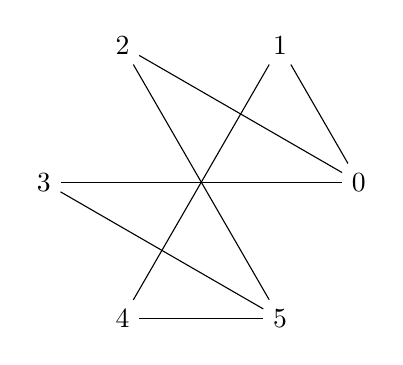
\begin{tikzpicture}
      \draw
        (0.0:2) node (0){0}
        (60.0:2) node (1){1}
        (120.0:2) node (2){2}
        (180.0:2) node (3){3}
        (240.0:2) node (4){4}
        (300.0:2) node (5){5};
      \begin{scope}[-]
        \draw (0) to (1);
        \draw (0) to (2);
        \draw (0) to (3);
        \draw (1) to (4);
        \draw (2) to (5);
        \draw (3) to (5);
        \draw (4) to (5);
      \end{scope}
    \end{tikzpicture}
\end{figure}
\begin{itemize}
\item signature: 111000010001011
\item g: Graph with 6 nodes and 7 edges
\item order: 6
\item size: 7
\item max degree: 3
\item degrees: 2,2,2,2,3,3
\item is tree: 0
\item is bipartite: 0
\item has bridge: 0
\item is chordal: 0
\item is complete: 0
\item min cycle basis weight: 9
\item min cycle basis size: 2
\item diameter: 2
\item radius: 2
\item is eulerian: 0
\item is planar: 1
\item number of faces: 3
\item is regular: 0
\item p3: 10
\item p4: 9
\item property hash: 10e530549749e8bfab385a5820e77a6be687266eb8555cb25ca81df74a6e0ff9
\end{itemize}
\newpage
\begin{figure}
  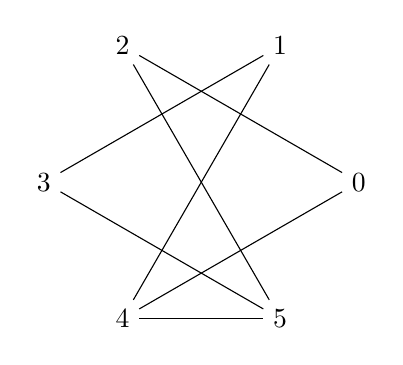
\begin{tikzpicture}
      \draw
        (0.0:2) node (0){0}
        (60.0:2) node (1){1}
        (120.0:2) node (2){2}
        (180.0:2) node (3){3}
        (240.0:2) node (4){4}
        (300.0:2) node (5){5};
      \begin{scope}[-]
        \draw (0) to (2);
        \draw (0) to (4);
        \draw (1) to (3);
        \draw (1) to (4);
        \draw (2) to (5);
        \draw (3) to (5);
        \draw (4) to (5);
      \end{scope}
    \end{tikzpicture}
\end{figure}
\begin{itemize}
\item signature: 010100110001011
\item g: Graph with 6 nodes and 7 edges
\item order: 6
\item size: 7
\item max degree: 3
\item degrees: 2,2,2,2,3,3
\item is tree: 0
\item is bipartite: 1
\item has bridge: 0
\item is chordal: 0
\item is complete: 0
\item min cycle basis weight: 8
\item min cycle basis size: 2
\item diameter: 3
\item radius: 2
\item is eulerian: 0
\item is planar: 1
\item number of faces: 3
\item is regular: 0
\item p3: 10
\item p4: 6
\item property hash: 0d37d15d2bdb8275d94a0f9aeca55ae56316027f7435ade215e6ecbc01bd531f
\end{itemize}
\newpage
\begin{figure}
  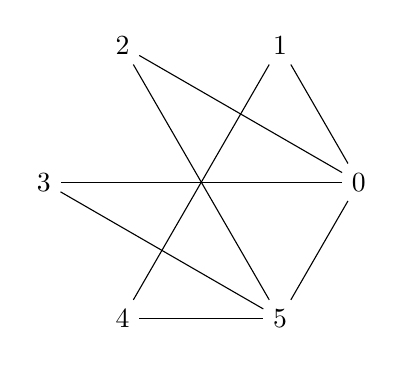
\begin{tikzpicture}
      \draw
        (0.0:2) node (0){0}
        (60.0:2) node (1){1}
        (120.0:2) node (2){2}
        (180.0:2) node (3){3}
        (240.0:2) node (4){4}
        (300.0:2) node (5){5};
      \begin{scope}[-]
        \draw (0) to (1);
        \draw (0) to (2);
        \draw (0) to (3);
        \draw (0) to (5);
        \draw (1) to (4);
        \draw (2) to (5);
        \draw (3) to (5);
        \draw (4) to (5);
      \end{scope}
    \end{tikzpicture}
\end{figure}
\begin{itemize}
\item signature: 111010010001011
\item g: Graph with 6 nodes and 8 edges
\item order: 6
\item size: 8
\item max degree: 4
\item degrees: 2,2,2,2,4,4
\item is tree: 0
\item is bipartite: 0
\item has bridge: 0
\item is chordal: 0
\item is complete: 0
\item min cycle basis weight: 10
\item min cycle basis size: 3
\item diameter: 2
\item radius: 2
\item is eulerian: 1
\item is planar: 1
\item number of faces: 4
\item is regular: 0
\item p3: 10
\item p4: None
\item property hash: aa044d77538b612d8b0e4f05d40ba57eea1d9c35ab0438fe2f5640380e5f2c04
\end{itemize}
\newpage
\begin{figure}
  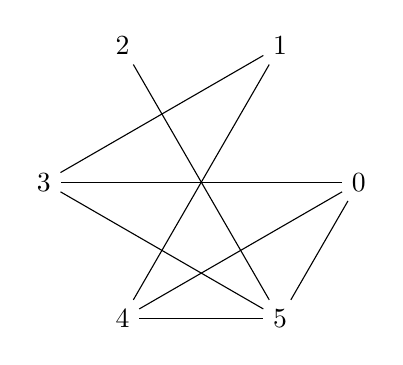
\begin{tikzpicture}
      \draw
        (0.0:2) node (0){0}
        (60.0:2) node (1){1}
        (120.0:2) node (2){2}
        (180.0:2) node (3){3}
        (240.0:2) node (4){4}
        (300.0:2) node (5){5};
      \begin{scope}[-]
        \draw (0) to (3);
        \draw (0) to (4);
        \draw (0) to (5);
        \draw (1) to (3);
        \draw (1) to (4);
        \draw (2) to (5);
        \draw (3) to (5);
        \draw (4) to (5);
      \end{scope}
    \end{tikzpicture}
\end{figure}
\begin{itemize}
\item signature: 001110110001011
\item g: Graph with 6 nodes and 8 edges
\item order: 6
\item size: 8
\item max degree: 4
\item degrees: 1,2,3,3,3,4
\item is tree: 0
\item is bipartite: 0
\item has bridge: 1
\item is chordal: 0
\item is complete: 0
\item min cycle basis weight: 10
\item min cycle basis size: 3
\item diameter: 3
\item radius: 2
\item is eulerian: 0
\item is planar: 1
\item number of faces: 4
\item is regular: 0
\item p3: 10
\item p4: None
\item property hash: 67db3380052eee413b1cc7745c9e67ca369f8cc31a3589b0359280de761b1a02
\end{itemize}
\newpage
\begin{figure}
  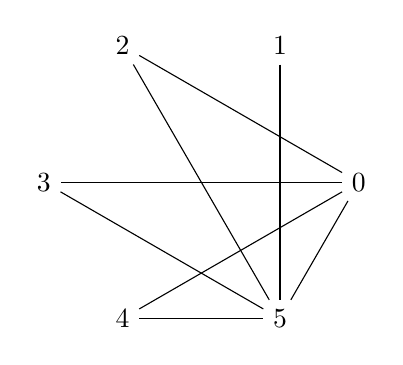
\begin{tikzpicture}
      \draw
        (0.0:2) node (0){0}
        (60.0:2) node (1){1}
        (120.0:2) node (2){2}
        (180.0:2) node (3){3}
        (240.0:2) node (4){4}
        (300.0:2) node (5){5};
      \begin{scope}[-]
        \draw (0) to (2);
        \draw (0) to (3);
        \draw (0) to (4);
        \draw (0) to (5);
        \draw (1) to (5);
        \draw (2) to (5);
        \draw (3) to (5);
        \draw (4) to (5);
      \end{scope}
    \end{tikzpicture}
\end{figure}
\begin{itemize}
\item signature: 011110001001011
\item g: Graph with 6 nodes and 8 edges
\item order: 6
\item size: 8
\item max degree: 5
\item degrees: 1,2,2,2,4,5
\item is tree: 0
\item is bipartite: 0
\item has bridge: 1
\item is chordal: 1
\item is complete: 0
\item min cycle basis weight: 9
\item min cycle basis size: 3
\item diameter: 2
\item radius: 1
\item is eulerian: 0
\item is planar: 1
\item number of faces: 4
\item is regular: 0
\item p3: 10
\item p4: None
\item property hash: a8d00518116224e982eb931c8caa7eb2627ed2ff638c9fc39e52606dbc90e70e
\end{itemize}
\newpage
\begin{figure}
  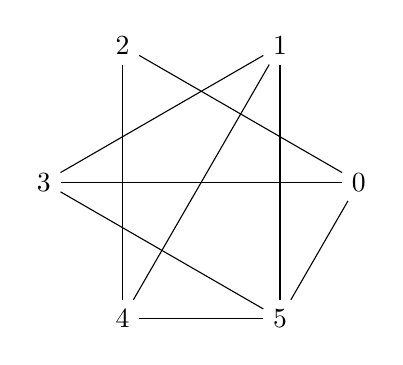
\begin{tikzpicture}
      \draw
        (0.0:2) node (0){0}
        (60.0:2) node (1){1}
        (120.0:2) node (2){2}
        (180.0:2) node (3){3}
        (240.0:2) node (4){4}
        (300.0:2) node (5){5};
      \begin{scope}[-]
        \draw (0) to (2);
        \draw (0) to (3);
        \draw (0) to (5);
        \draw (1) to (3);
        \draw (1) to (4);
        \draw (1) to (5);
        \draw (2) to (4);
        \draw (3) to (5);
        \draw (4) to (5);
      \end{scope}
    \end{tikzpicture}
\end{figure}
\begin{itemize}
\item signature: 011010111010011
\item g: Graph with 6 nodes and 9 edges
\item order: 6
\item size: 9
\item max degree: 4
\item degrees: 2,3,3,3,3,4
\item is tree: 0
\item is bipartite: 0
\item has bridge: 0
\item is chordal: 0
\item is complete: 0
\item min cycle basis weight: 13
\item min cycle basis size: 4
\item diameter: 2
\item radius: 2
\item is eulerian: 0
\item is planar: 1
\item number of faces: 5
\item is regular: 0
\item p3: 10
\item p4: 7
\item property hash: 8ee4ab9d43d3defabeb45d0226efb1fdd7518b770a2ff45d44da3f2c79510c59
\end{itemize}
\newpage
\begin{figure}
  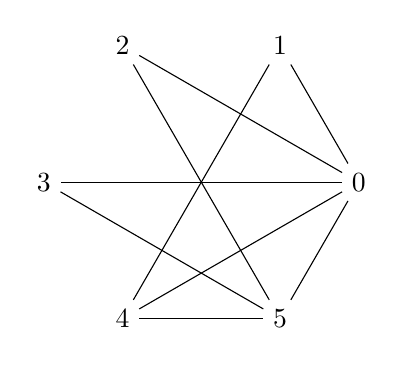
\begin{tikzpicture}
      \draw
        (0.0:2) node (0){0}
        (60.0:2) node (1){1}
        (120.0:2) node (2){2}
        (180.0:2) node (3){3}
        (240.0:2) node (4){4}
        (300.0:2) node (5){5};
      \begin{scope}[-]
        \draw (0) to (1);
        \draw (0) to (2);
        \draw (0) to (3);
        \draw (0) to (4);
        \draw (0) to (5);
        \draw (1) to (4);
        \draw (2) to (5);
        \draw (3) to (5);
        \draw (4) to (5);
      \end{scope}
    \end{tikzpicture}
\end{figure}
\begin{itemize}
\item signature: 111110010001011
\item g: Graph with 6 nodes and 9 edges
\item order: 6
\item size: 9
\item max degree: 5
\item degrees: 2,2,2,3,4,5
\item is tree: 0
\item is bipartite: 0
\item has bridge: 0
\item is chordal: 1
\item is complete: 0
\item min cycle basis weight: 12
\item min cycle basis size: 4
\item diameter: 2
\item radius: 1
\item is eulerian: 0
\item is planar: 1
\item number of faces: 5
\item is regular: 0
\item p3: 10
\item p4: None
\item property hash: e8b4b026d011e396640daa02d06681fd9422455e343a8be4072c1f1b5056fb29
\end{itemize}
\newpage
\begin{figure}
  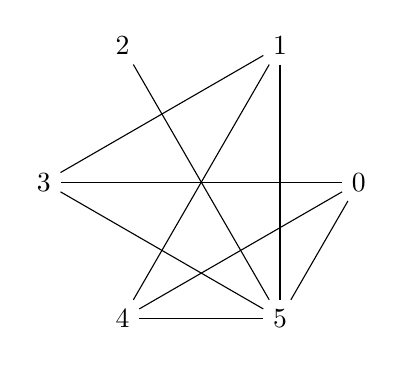
\begin{tikzpicture}
      \draw
        (0.0:2) node (0){0}
        (60.0:2) node (1){1}
        (120.0:2) node (2){2}
        (180.0:2) node (3){3}
        (240.0:2) node (4){4}
        (300.0:2) node (5){5};
      \begin{scope}[-]
        \draw (0) to (3);
        \draw (0) to (4);
        \draw (0) to (5);
        \draw (1) to (3);
        \draw (1) to (4);
        \draw (1) to (5);
        \draw (2) to (5);
        \draw (3) to (5);
        \draw (4) to (5);
      \end{scope}
    \end{tikzpicture}
\end{figure}
\begin{itemize}
\item signature: 001110111001011
\item g: Graph with 6 nodes and 9 edges
\item order: 6
\item size: 9
\item max degree: 5
\item degrees: 1,3,3,3,3,5
\item is tree: 0
\item is bipartite: 0
\item has bridge: 1
\item is chordal: 0
\item is complete: 0
\item min cycle basis weight: 12
\item min cycle basis size: 4
\item diameter: 2
\item radius: 1
\item is eulerian: 0
\item is planar: 1
\item number of faces: 5
\item is regular: 0
\item p3: 10
\item p4: None
\item property hash: 733375904d8af4120896b8d587913b61d232bb0e93988a5ce410e3ec4f3c72d4
\end{itemize}
\newpage
\begin{figure}
  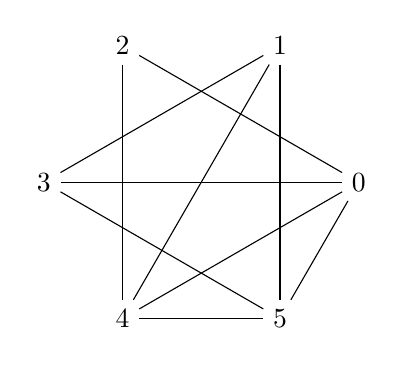
\begin{tikzpicture}
      \draw
        (0.0:2) node (0){0}
        (60.0:2) node (1){1}
        (120.0:2) node (2){2}
        (180.0:2) node (3){3}
        (240.0:2) node (4){4}
        (300.0:2) node (5){5};
      \begin{scope}[-]
        \draw (0) to (2);
        \draw (0) to (3);
        \draw (0) to (4);
        \draw (0) to (5);
        \draw (1) to (3);
        \draw (1) to (4);
        \draw (1) to (5);
        \draw (2) to (4);
        \draw (3) to (5);
        \draw (4) to (5);
      \end{scope}
    \end{tikzpicture}
\end{figure}
\begin{itemize}
\item signature: 011110111010011
\item g: Graph with 6 nodes and 10 edges
\item order: 6
\item size: 10
\item max degree: 4
\item degrees: 2,3,3,4,4,4
\item is tree: 0
\item is bipartite: 0
\item has bridge: 0
\item is chordal: 0
\item is complete: 0
\item min cycle basis weight: 15
\item min cycle basis size: 5
\item diameter: 2
\item radius: 2
\item is eulerian: 0
\item is planar: 1
\item number of faces: 6
\item is regular: 0
\item p3: 10
\item p4: None
\item property hash: f04dbaadc9b3ebc08bffff0dc64f81edd9ab5fa64aa0ad421b12478ca02352d6
\end{itemize}
\newpage
\begin{figure}
  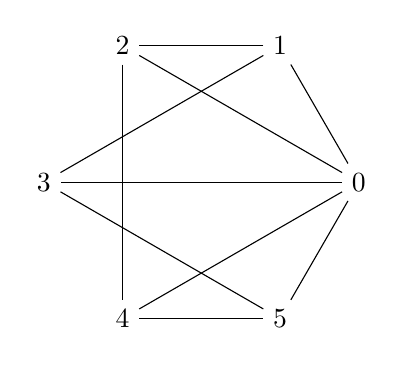
\begin{tikzpicture}
      \draw
        (0.0:2) node (0){0}
        (60.0:2) node (1){1}
        (120.0:2) node (2){2}
        (180.0:2) node (3){3}
        (240.0:2) node (4){4}
        (300.0:2) node (5){5};
      \begin{scope}[-]
        \draw (0) to (1);
        \draw (0) to (2);
        \draw (0) to (3);
        \draw (0) to (4);
        \draw (0) to (5);
        \draw (1) to (2);
        \draw (1) to (3);
        \draw (2) to (4);
        \draw (3) to (5);
        \draw (4) to (5);
      \end{scope}
    \end{tikzpicture}
\end{figure}
\begin{itemize}
\item signature: 111111100010011
\item g: Graph with 6 nodes and 10 edges
\item order: 6
\item size: 10
\item max degree: 5
\item degrees: 3,3,3,3,3,5
\item is tree: 0
\item is bipartite: 0
\item has bridge: 0
\item is chordal: 0
\item is complete: 0
\item min cycle basis weight: 15
\item min cycle basis size: 5
\item diameter: 2
\item radius: 1
\item is eulerian: 0
\item is planar: 1
\item number of faces: 6
\item is regular: 0
\item p3: 10
\item p4: None
\item property hash: 6d0a08989b3607678606bfbe7420ffd842ee47ae25e431cf8f0f037600fb3995
\end{itemize}
\newpage
\begin{figure}
  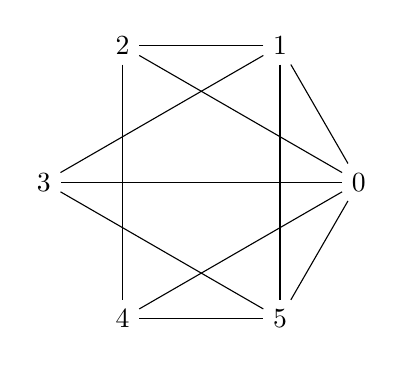
\begin{tikzpicture}
      \draw
        (0.0:2) node (0){0}
        (60.0:2) node (1){1}
        (120.0:2) node (2){2}
        (180.0:2) node (3){3}
        (240.0:2) node (4){4}
        (300.0:2) node (5){5};
      \begin{scope}[-]
        \draw (0) to (1);
        \draw (0) to (2);
        \draw (0) to (3);
        \draw (0) to (4);
        \draw (0) to (5);
        \draw (1) to (2);
        \draw (1) to (3);
        \draw (1) to (5);
        \draw (2) to (4);
        \draw (3) to (5);
        \draw (4) to (5);
      \end{scope}
    \end{tikzpicture}
\end{figure}
\begin{itemize}
\item signature: 111111101010011
\item g: Graph with 6 nodes and 11 edges
\item order: 6
\item size: 11
\item max degree: 5
\item degrees: 3,3,3,4,4,5
\item is tree: 0
\item is bipartite: 0
\item has bridge: 0
\item is chordal: 0
\item is complete: 0
\item min cycle basis weight: 18
\item min cycle basis size: 6
\item diameter: 2
\item radius: 1
\item is eulerian: 0
\item is planar: 1
\item number of faces: 7
\item is regular: 0
\item p3: 10
\item p4: None
\item property hash: 1c0d3025906190d63406c105289f470203d11fd43e753a1b04e6241b5bac19bd
\end{itemize}
\newpage
